% Этот текст можно свободно редактировать.
\FloatBarrier
\section{Устойчивость и анализ}

\FloatBarrier
\begingroup
\setlength{\tabcolsep}{3pt}
\setlength{\reporttablewidth}{\dimexpr\linewidth-18pt\relax}
\renewcommand{\arraystretch}{1.15}
\small
\begin{longtable}{@{}>{\raggedright\arraybackslash}p{0.25000\reporttablewidth}>{\raggedright\arraybackslash}p{0.25000\reporttablewidth}>{\raggedright\arraybackslash}p{0.25000\reporttablewidth}>{\raggedright\arraybackslash}p{0.25000\reporttablewidth}@{}}
\caption{Устойчивость и анализ}\label{tab:results-6}\\
\toprule
\textbf{Кандидаты} & \textbf{Модель} & \textbf{NDCG@10} & \textbf{Recall@10} \\
\midrule
\endfirsthead
\multicolumn{4}{l}{\small\itshape Продолжение таблицы \thetable}\\
\toprule
\textbf{Кандидаты} & \textbf{Модель} & \textbf{NDCG@10} & \textbf{Recall@10} \\
\midrule
\endhead
\midrule
\multicolumn{4}{r}{\footnotesize Продолжение на следующей странице}\\
\endfoot
\bottomrule
\endlastfoot
mixed & Ручные признаки & 0.47332 & 0.71530 \\
mixed & Автоотбор & 0.48440 & 0.71821 \\
uniform & Ручные признаки & 0.68320 & 0.87864 \\
uniform & Автоотбор & 0.68729 & 0.87999 \\
полный каталог, 210 запросов & Ручные признаки & 0.09875 & 0.16825 \\
полный каталог, 210 запросов & Автоотбор & 0.10332 & 0.17873 \\
полный каталог, 210 запросов & Популярность, 7 дней & 0.14847 & 0.23294 \\
\end{longtable}
\endgroup

В режиме uniform меняются только отрицательные кандидаты: все они равномерные. Модели и выбор признаков зафиксированы заранее, до открытия теста. Сдвиг распределения контролей означает, что LogLoss этого режима требует отдельной интерпретации; основное внимание --- ранжированию.

Проверка полного каталога: \textbf{210 случайных тестовых запросов}, выбор без возвращения с seed 2026. Для каждого ранжируется \textbf{весь} ранее наблюдавшийся каталог за исключением уже виденных пользователем объектов; контрольные объекты не сэмплируются. Это всё ещё каталог выбранных 30 000 пользователей, а не весь бизнес-каталог KION. Полный список запросов, размеры каталога по дням и доверительный интервал находятся в \code{full_catalog.json}. Сравнение на этом подмножестве не заменяет полный тест по всем запросам; интервал обычно шире. Для каталожной разницы получено +0.00456, 95\% ДИ [-0.01240, +0.02253]. На полном каталоге положительная разность статистически не подтверждена: интервал включает ноль.

\FloatBarrier
\begingroup
\setlength{\tabcolsep}{3pt}
\setlength{\reporttablewidth}{\dimexpr\linewidth-24pt\relax}
\renewcommand{\arraystretch}{1.15}
\small
\begin{longtable}{@{}>{\raggedright\arraybackslash}p{0.20000\reporttablewidth}>{\raggedright\arraybackslash}p{0.20000\reporttablewidth}>{\raggedright\arraybackslash}p{0.20000\reporttablewidth}>{\raggedright\arraybackslash}p{0.20000\reporttablewidth}>{\raggedright\arraybackslash}p{0.20000\reporttablewidth}@{}}
\caption{Устойчивость и анализ}\label{tab:results-7}\\
\toprule
\textbf{Модель} & \textbf{Тёплые запросы} & \textbf{NDCG@10 warm} & \textbf{Холодные запросы} & \textbf{NDCG@10 cold} \\
\midrule
\endfirsthead
\multicolumn{5}{l}{\small\itshape Продолжение таблицы \thetable}\\
\toprule
\textbf{Модель} & \textbf{Тёплые запросы} & \textbf{NDCG@10 warm} & \textbf{Холодные запросы} & \textbf{NDCG@10 cold} \\
\midrule
\endhead
\midrule
\multicolumn{5}{r}{\footnotesize Продолжение на следующей странице}\\
\endfoot
\bottomrule
\endlastfoot
Ручные признаки & 6258 & 0.45852 & 1720 & 0.52720 \\
Автоотбор & 6258 & 0.46894 & 1720 & 0.54064 \\
\end{longtable}
\endgroup

Cold --- пользователь без записей строго до даты запроса, даже если его ID был выбран из общей выгрузки. Такой пользователь не исключается из оценки. У него нет истории для косвенных признаков; доступны справочник, календарь и глобальная популярность. Объекты с нулевой историей на дату прогноза исключены. Объекты, не встречавшиеся при обучении, но появившиеся в последующей доступной истории, могут попасть в каталог; отдельная метрика этого среза не вычислялась. Это ограничивает выводы о cold-start объектов.

У cold-среза здесь NDCG выше, чем у warm. Это не причинный эффект отсутствия истории: запросы и целевые объекты двух групп различаются, а cold определяется по доступным записям выгрузки, не по дате регистрации аккаунта. Сравнивать полезность истории следует по контролируемой абляции, а не по разности этих двух популяционных средних.

\FloatBarrier
\begingroup
\setlength{\tabcolsep}{3pt}
\setlength{\reporttablewidth}{\dimexpr\linewidth-6pt\relax}
\renewcommand{\arraystretch}{1.15}
\small
\begin{longtable}{@{}>{\raggedright\arraybackslash}p{0.17647\reporttablewidth}>{\raggedright\arraybackslash}p{0.82353\reporttablewidth}@{}}
\caption{Устойчивость и анализ}\label{tab:results-8}\\
\toprule
\textbf{Модель} & \textbf{Самые важные признаки, в порядке убывания} \\
\midrule
\endfirsthead
\multicolumn{2}{l}{\small\itshape Продолжение таблицы \thetable}\\
\toprule
\textbf{Модель} & \textbf{Самые важные признаки, в порядке убывания} \\
\midrule
\endhead
\midrule
\multicolumn{2}{r}{\footnotesize Продолжение на следующей странице}\\
\endfoot
\bottomrule
\endlastfoot
Ручные признаки & \code{item_recency}, \code{item__count__30d}, \code{item__count__7d}, \code{item__count__0d}, \code{item_id}, \code{user_type__share__0d}, \code{user_genre__share__0d}, \code{user_country__share__0d} \\
Автоотбор & \code{item__ewm__h2}, \code{item_recency}, \code{item__count__30d}, \code{item__count__0d}, \code{item__count__3d}, \code{item_id}, \code{item__count__7d}, \code{user_genre__share__0d} \\
\end{longtable}
\endgroup

\begin{figure}[!htbp]
\centering
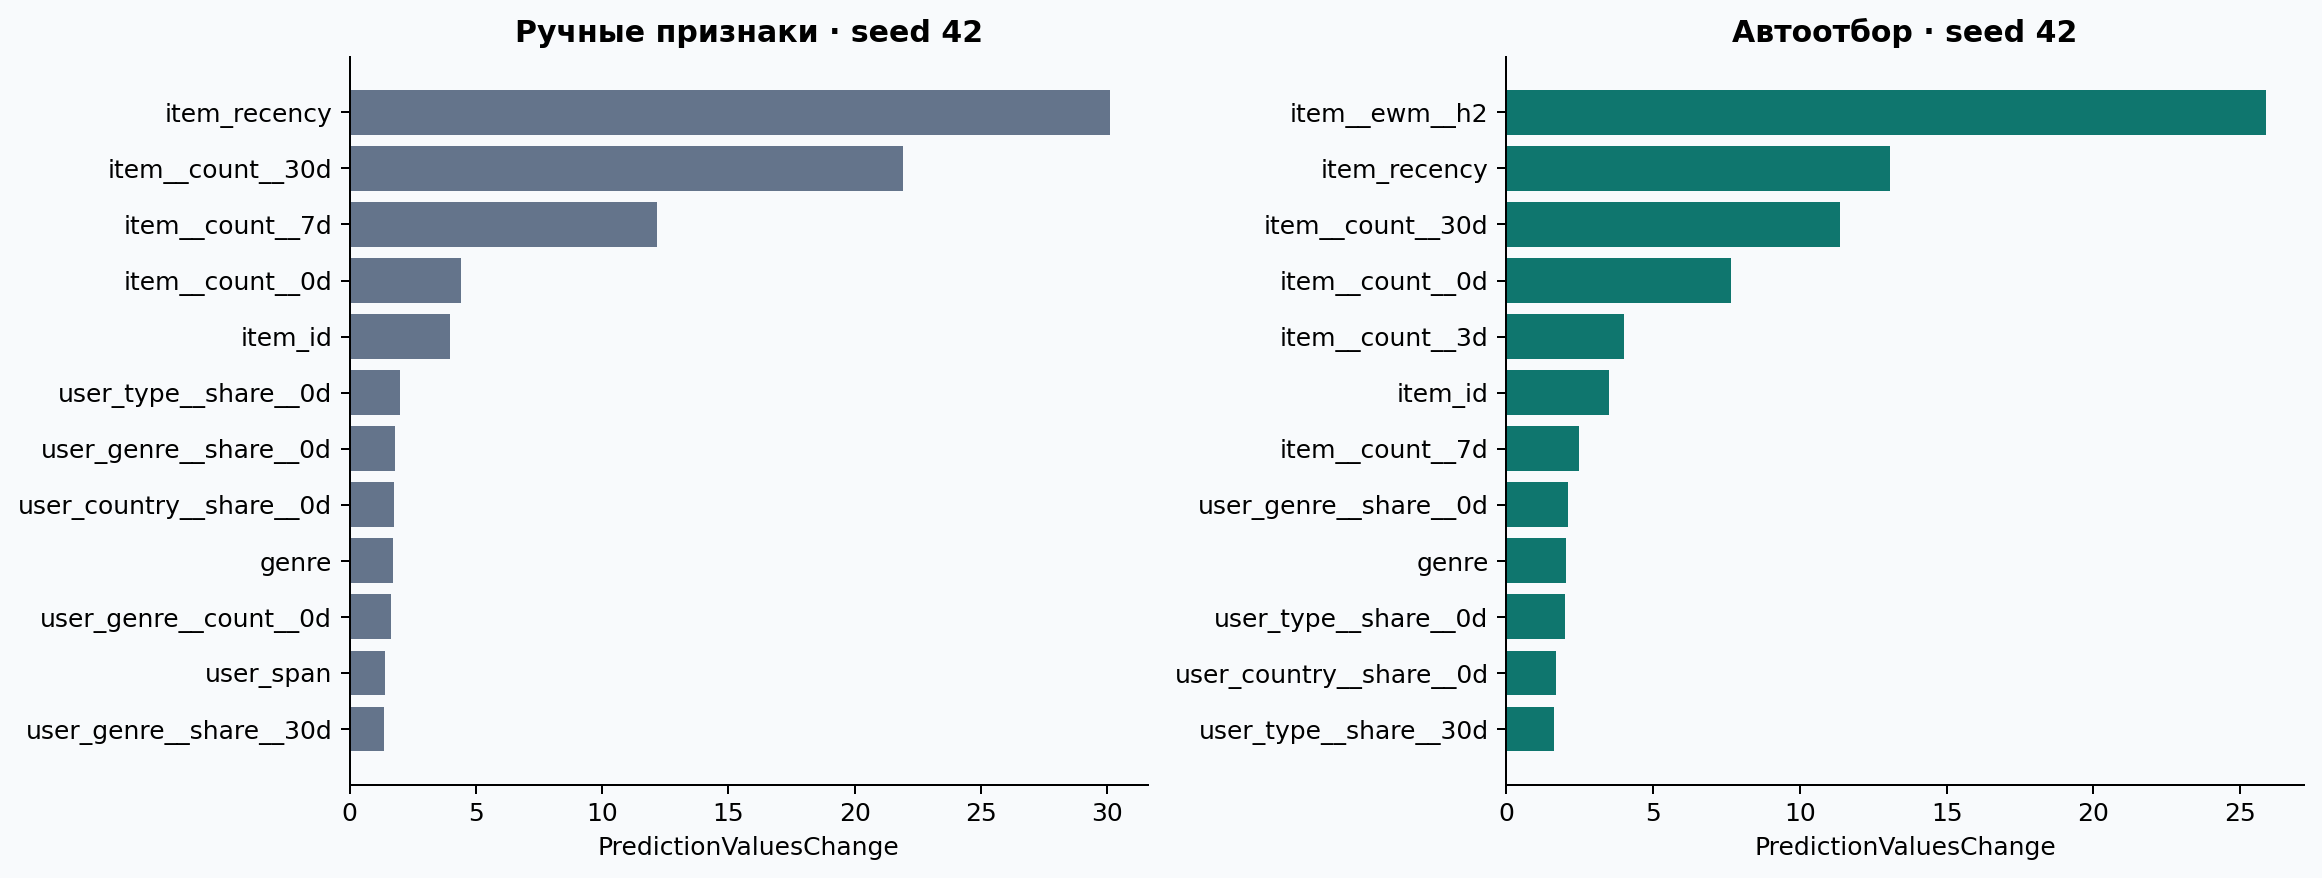
\includegraphics[width=\linewidth,height=.70\textheight,keepaspectratio]{figures/importance.png}
\caption{Важность признаков}
\label{fig:importance}
\end{figure}
Важности --- \code{PredictionValuesChange}, они описывают использование признаков моделью, а не причинный эффект. Коррелирующие окна делят важность. Контролируемые абляции содержательнее одной картинки: удаление косвенных исторических связей даёт NDCG@10=0.42575, весь банк без отбора --- 0.49114. Для точного сравнения отдельных компонентов нужно смотреть одноимённые seed 42, а не смешивать их с ансамблем. Поиск оценивает и неудачные группы; отсутствие прироста группы на search не доказывает её бесполезность на другом объёме данных или другом датасете.

При одном seed 42 добавление косвенных исторических связей меняет NDCG@10 на \textbf{+0.04355} относительно абляции без них. Замена всего автоматического банка выбранным подмножеством меняет метрику на \textbf{-0.00746}. Эти одноразовые абляционные разности описательные: отдельные доверительные интервалы для них не вычислялись.

Полный банк оказался не хуже отобранного набора при одном seed. Возможная причина - поиск на 180 деревьях и не более трёх групп не отражает все взаимодействия при полном бюджете; причинное объяснение этим экспериментом не установлено.

Это была исходная гипотеза. Её контролируемая проверка через изменение только лимита деревьев приведена в §10.2; окончательный вывод о механизме следует брать из этой проверки.

В полном банке \code{item__ewm__h10} имеет высокую важность, хотя группа decay\_10d не вошла в лучший короткий поиск; существенен и \code{genre_affinity_mean}. Это описательное свидетельство того, что ранжирование групп на 180 деревьях недостаточно для выбора всех полезных сочетаний на 450 деревьях. Важность не доказывает индивидуальную причинную пользу: для неё нужна отдельная абляция на новом независимом периоде.

\FloatBarrier
\subsection*{Почему полный каталог дал другой вывод}
\addcontentsline{toc}{subsection}{Почему полный каталог дал другой вывод}

Популярность за 7 дней описательно сильнее обеих обученных моделей на проверенных 210 запросах. Для разницы с популярностью отдельный статистический тест не проводился; основной каталожный интервал относится к автоотбору против ручного CatBoost. Классификатор оптимизировался на сэмплированных кандидатах, и такой результат нельзя подавать как победу в каталожном retrieval.

Одна проверяемая гипотеза --- влияние распределения контролей. В идеализированной бинарной задаче odds оптимального классификатора пропорциональны \code{p_positive(item|context) / q_negative(item|context)}. При неравномерном q ранжирование raw score не обязано совпадать с ранжированием частоты позитивного события. Эта логика связана с \href{https://proceedings.mlr.press/v9/gutmann10a.html}{data-vs-noise классификацией}. В нашем генераторе половина контролей зависит от популярности, а выбор без возвращения и исключения дополнительно усложняют точные вероятности включения. Коррекция по ним не применялась. Ещё возможны влияние редких историй и устаревших категориальных зависимостей; эти причины не отделены экспериментом.

Следующий независимый эксперимент должен включать каталожную валидацию, другой закон контролей или корректно выведенную поправку на сэмплирование. Исходные модели и их параметры после просмотра этого теста не менялись. Дополнительные обучения и проверки из §10 зафиксированы отдельно; каталожный результат не использован для смены признаков или закона контролей.

